\chapter{Élaboration  et évaluation du modèle de prédiction }
Tous au long de ce chapitre nous allons entrainer nos algorithmes de prédiction avec des données provenant de chaque faculté et essayerons de prédire le CGPA, nous  avons utiliser des algorithmes présenté au chapitre premier pour entrainer nos modèles de prédiction.
Pour choisir l'algorithme à utiliser nous somme basée sur la documentation officielle de la librairie scikit-learn \cite{pedregosa2011scikit} qui nous a fourni l'infographie sur la figure \ref{fig:skLearn1} pour le choix des algorithmes. \\

\begin{figure}[ht]
	\centering
	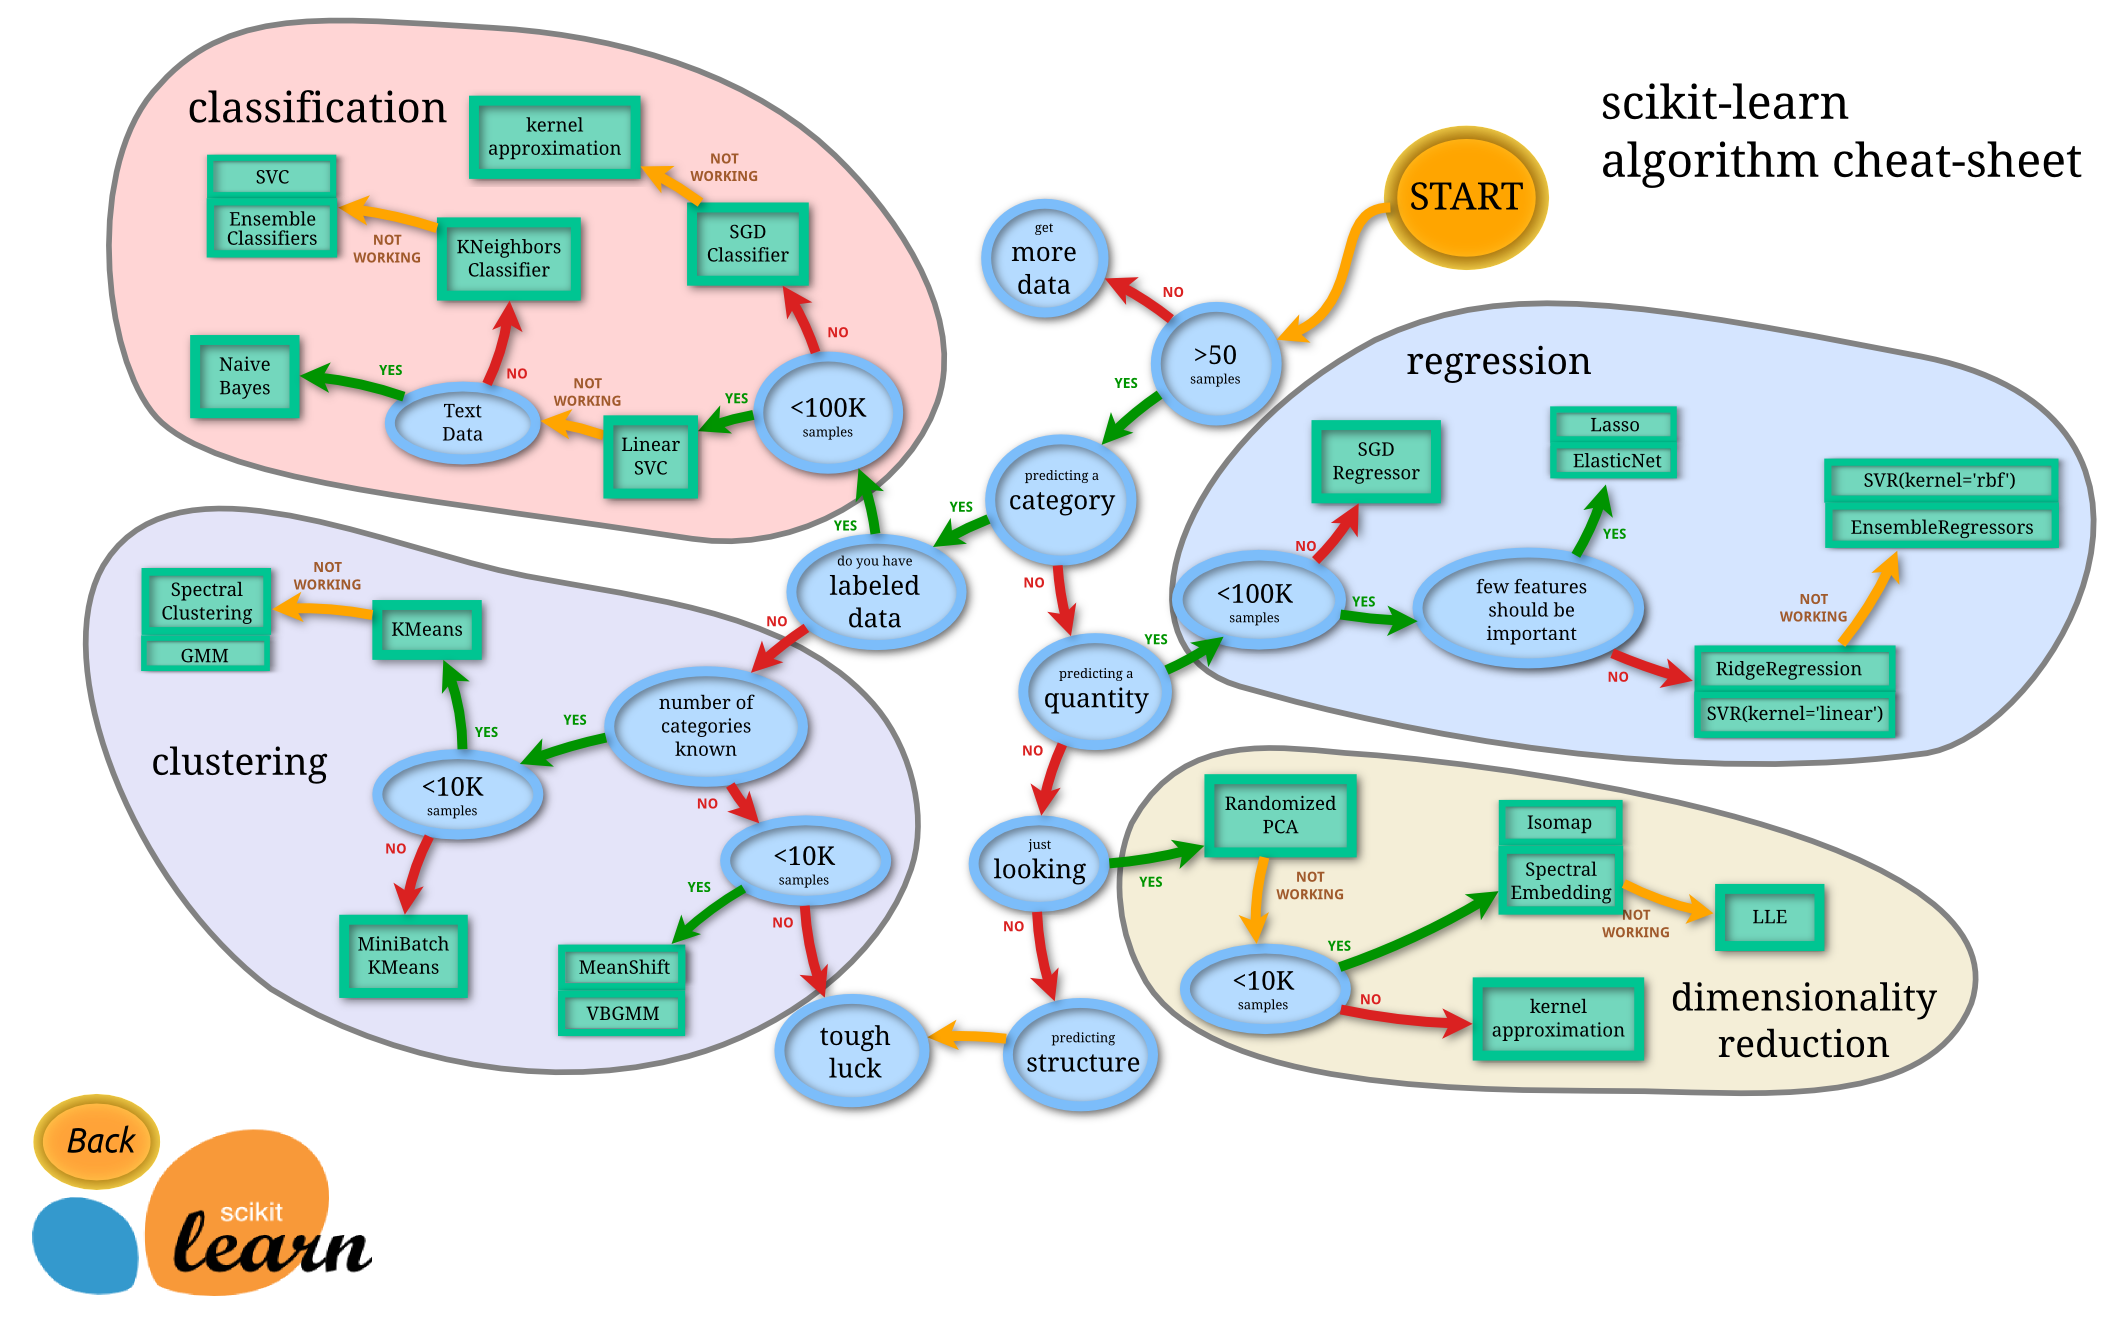
\includegraphics[width=0.5\textwidth]{fig/sckikLearnCheatSheet.png}
	\caption[Short caption]{sckit-Learn Algorithm cheat sheet }
	\label{fig:skLearn1}
\end{figure} 

Vu que nous disposons de moins de 100000 instances pour nos ensemble d'apprentissage et vu que notre tache était celui de prédire une variable continue (Une régression )  nous avions décidé d'entrainer les algorithmes  suivantes :
\begin{enumerate}
	\item Ridge Régression
	\item Elastic Net Régression
	\item Lasso Régression
	\item \ac{SVR} avec Kernel Linéaire
	\item  \ac{SVR} avec Kernel Gaussien 
\end{enumerate}
Les 3 premiers modèles sont des versions issues de la régularisation de la régression linéaire vu au chapitre 1  et qui conviennent bien pour des ensembles d'apprentissages relativement petits , le 2 derniers sont une adaptation du \ac{SVM} pour la régression.\\
Notons que toutes ses librairies sont bien implémentées et optimisées dans scikit-learn.
Tous au long de ce chapitre nous avions suivie les étapes suivantes  sur la figure \ref{fig:predictiveModelBuilding}:
 \begin{enumerate}
 \item Préparation des données :
 \begin{itemize}
 	\item  Encodage One Hot
 	\item  Normalisation
 	\item  Échantillonnage
 \end{itemize}
\item Exécution des algorithmes
\item évaluation 
   \begin{itemize}
  	\item  Évaluation sur l'ensemble d'apprentissage (training set)
  	\item  Validation croisée sur l'ensemble d'apprentissage
  	\item  Évaluation sur l'ensemble d'évaluation (test set) 
  \end{itemize}
\item Amélioration des modèles par les méthodes d'ensembles
\item Évaluation du modèle finale
 \end{enumerate}
\begin{figure}[ht]
	\centering
	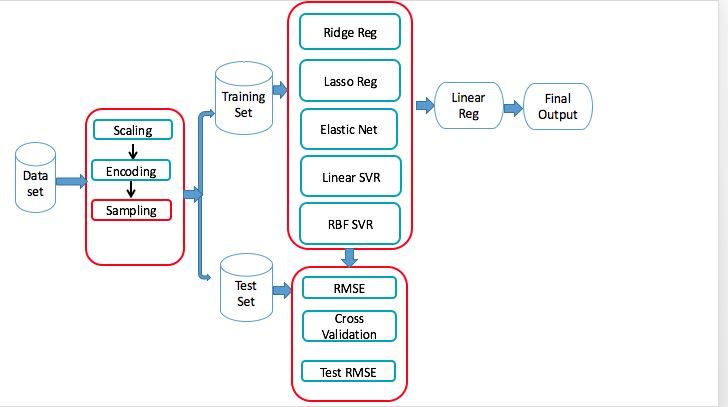
\includegraphics[width=0.5\textwidth]{fig/ModelBuilding.png}
	\caption[Short caption]{étapes à suivre pour l'élaboration du modèle d'apprentissage }
	\label{fig:predictiveModelBuilding}
\end{figure} 
\section {Préparation des données pour l'exécution des algorithmes } 
Dans cette partie nous expliquerons comment s'est passé la préparation des nos données , rappelons que notre ensemble d'apprentissage finale dispose de 4 attribues et notre valeur à prédire :
\begin{enumerate}
	\item  SCHOOLNAME : de nature catégorielle (string)
	\item  OPTION : de nature catégorielle (string)
	\item  DIPPERC : de nature continue (float)
	\item  CGPA : de nature continue (float)
\end{enumerate}
Comme l'a souligné \cite{OneHotEncoding} la librairie scikit learn ne travaille qu'avec les variables numériques , c'est pourquoi nous avions décider de transformer nos variables catégorielles les chaines de caractères en variables numériques en utilisant la technique du \emph{\textbf{One Hot encoding}} 
\subsection{Encodage des Variables One Hot }
Un encodage one-hot consiste à représenter des états en utilisant pour chacun une valeur dont la représentation binaire n'a qu'un seul chiffre 1.

On peut définir une fonction d'encodage one-hot comme étant la fonction qui prend en entrée un vecteur  z et qui redéfinit en sortie la plus grande valeur de  z à 1 et toutes autres valeurs de  z à 0.
L'avantage principal de cet encodage est que pour passer d'un état à un autre, seules deux transitions sont nécessaires : un chiffre passe de 1 à 0, un autre de 0 à 1. Son inconvénient est qu'il faut au minimum n bits pour représenter n états, ce qui conduit à une augmentation linéaire du nombre de chiffres par rapport au nombre d'états. Un encodage utilisant toutes les valeurs binaires existantes a quant à lui une augmentation logarithmique du nombre de chiffres.

Pour notre ensemble , après notre encodage nous pouvons aisément remarquer que notre ensemble d'apprentissage vient de passer de (4715, 4 )à (4715 , 647)  dimensions.
Mais ces dimension restent raisonnables pour un projet de machine Learning. 
\subsection{Normalisation  } 
Nous avions ensuite normaliser nos données pour les variables numérique en divisant le pourcentage du diplôme d'état par 100 et celui du CGPA,ceci pour permettre une exécution rapide de nos algorithmes. 
\subsection{Échantillonnage  \cite{statBook1} } 
Pour commencer notre entrainement nous avions échantillonner nos donnes pour constituer un ensemble d'apprentissage (Training set), et un ensemble d'évaluation du modèle (test set). Notre Training set était constituer de 80 \% de nos données et les 20 autres pour cent ont constitué notre ensemble d'évaluation.
Pour ce faire nous avions utilisé un échantillonnage stratifié.
Lorsqu'on utilise l'échantillonnage stratifié, on divise la population en groupes homogènes (appelés strates), qui sont mutuellement exclusifs, puis on sélectionne à partir de chaque strate des échantillons indépendants. On peut utiliser n'importe quelle des méthodes d'échantillonnage  pour sélectionner l'échantillon à l'intérieur de chaque strate. La méthode d'échantillonnage peut varier d'une strate à une autre. Lorsqu'on utilise l'échantillonnage aléatoire simple pour sélectionner l'échantillon à l'intérieur de chaque strate, on appelle le plan d'échantillonnage un plan d'échantillonnage aléatoire simple stratifié. On peut stratifier avant l'échantillonnage une population au moyen de toute variable dont on dispose pour la totalité des unités , pour notre étude nous avions utilisé la variable \textbf{EchecRatio}.

A la fin de cette phase nous avions pu obtenir un ensemble d'apprentissage (Training Set) et Un ensemble d'évaluation (Test Set )

\section {Élaboration et Évaluation du Modèle de Prédiction au sein de Chaque faculté} 
Dans cette section nous allons entrainer les différents algorithmes de prédictions avec les données de issue de chaque faculté et ensuite nous évaluerons le modèles sur les 2 ensemble.

Mais avant d'attaquer l'entrainement de nos modèle nous expliquerons nos métriques d'évaluations.
\subsection{Techniques D'évaluation} 
\subsubsection{\ac{RMSE} \cite{ProbaStat} }
C'est la racine carrée de la somme des carrées des différences entres les valeurs exactes et celles prédite par un modèle de prédiction pour chaque élément d'un ensemble d'apprentissage .
Il se donne par la formule suivante  :

 $RMSE=\sqrt{\frac{\sum _{=1}^{N}{\left[{h}_{\theta}\left({x}^{(i)}\right) - {y}^{(i)}\right]}^2} {N}}$
 
 Il constituera notre métrique d'évaluation pour tous nos modèles.
\subsubsection{Validation Croisé  \cite{CrossValidation}}
La validation croisée (« cross-validation ») est une méthode d’estimation de fiabilité d’un modèle fondé sur une technique d’échantillonnage. En fait, il y a au moins trois techniques de validation croisée : « test set validation » ou « holdout method », « k-fold cross-validation » et \ac{LOOCV} .
\begin{itemize}
	\item La première méthode est très simple, il suffit de diviser l'échantillon de taille n en deux sous échantillons, le premier d'apprentissage (communément supérieur à 60 \% de l'échantillon) et le second de test. Le modèle est bâti sur l'échantillon d'apprentissage et validé sur l'échantillon de test. L'erreur est estimée en calculant un test, une mesure ou un score de performance du modèle sur l'échantillon de test, par exemple l'erreur quadratique moyenne.
	\item Dans la seconde, on divise l'échantillon original en k échantillons, puis on sélectionne un des k échantillons comme ensemble de validation et les (k-1) autres échantillons constitueront l'ensemble d'apprentissage. On calcule comme dans la première méthode le score de performance. Puis on répète l'opération en sélectionnant un autre échantillon de validation parmi les (k-1) échantillons qui n'ont pas encore été utilisés pour la validation du modèle. L'opération se répète ainsi k fois pour qu'en fin de compte chaque sous-échantillon ait été utilisé exactement une fois comme ensemble de validation. La moyenne des k erreurs quadratiques moyennes est enfin calculée pour estimer l'erreur de prédiction. 
	\item La troisième méthode est un cas particulier de la deuxième méthode où k=n, c'est-à-dire que l'on apprend sur (n-1) observations puis on valide le modèle sur la énième observation et l'on répète cette opération n fois . 
\end{itemize}

Tous au long de ce chapitre nous avions utilisé les 2 premières techniques , nous n'avions pas utiliser le 3 ème car elle est trop gourmande  en terme de ressource(temps et mémoire) 

Nous pouvons maintenant attaquer l'entrainement des modèles au sein de chaque faculté  :
\subsection{Résultat des différents algorithmes par faculté}
Le tableau qui va suivre décrira les différentes algorithmes que nous avions entrainer pour les données de chaque faculté , chaque modèles dispose des paramètres ainsi que des différentes erreurs.
 \newpage
\begin{table} [!htbp]
	\begingroup % make the next setting local
	\captionsetup{type=table} % here we want to caption a table
	\caption{Résultat des Algorithmes }
	\label{tab:AlgoResults}
	\noindent
	{\resizebox*{\textwidth}{\textheight}{%
			\renewcommand{\arraystretch}{2}
	\begin{tabular}{|c|c|c|c|c|c|c|c|}
		\toprule
		\multirow{6}{*}{} Faculté & Dimensions &Modèle&Paramètres &RMSE Train &\multicolumn{2}{c|}{CV Score}&RMSE Test  \\
		\cline{6-7}
		&&&&&M&std& \\
		\cline{1-8}
		\hline
		&&Ridge&alpha=1 , solver=cholesky &0.047:8\%&0.064:11\%&0.01&0.066:11.42\% \\
		&&Lasso&${\alpha}$=1e-05,iIter=10000&0.040 :  7.04\%&0.0640 :11.11\%&0.008& 0.068 : 11.93\%\\
		\cline{3-8}
		Médecine&{242 x 111 }&Elastic Net&${\alpha}$=1e-05, Iter=10000, l1Ratio=1&0.040 : 7.04\%&0.0641:11.115\%&0.0089&0.069 :11.97\% \\
		\cline{3-8}
		&&LinearSVR&Kernel=Linear&0.044:7.7\%&0.066:11\%&0.01& 0.08 : 13\%\\
		\cline{3-8}
		&&RbfSVR&Kernel = Gaussian&0.06788 :  11.76\%&0.0712:12.35\%&0.0084&0.062 : 10.74\% \\
		\cline{1-8}
		\hline
		\multirow{5}{*}{}
		&&Elastic Net&${\alpha}$=1e-05,Iter=10000,l1Ratio=1&0.078 :14.2\%&0.080 :14.54\%&0.0067& 0.078 : 14.21\%\\
		\cline{3-8}
		&&Lasso&${\alpha}$=1e-05,iIter=10000&0.0784 : 14.15\%&0.080 :14.49\%& 0.006&0.0784 : 14.15\% \\
		\cline{3-8}
		Technologie&{903x240}&Ridge&${\alpha}$=1 ,solver=cholesky&0.076 :13.83\% &0.07732 : 13.95\%&0.0066&0.076: 13.83\% \\
		\cline{3-8}
		&&LinearSVR&kernel=linear&0.0774 : 13.97\%&0.081:14.75\%&0.006& 0.077 :13.97\%\\
		\cline{3-8}
		&&RbfSVR&Kernel =Gaussian&0.0772  :  13.94\%&0.0798 :14.41\%&0.0053& 0.077 : 13.94\%\\
		\cline{1-8}
		\hline
		\multirow{5}{*}{}
		&&Elastic Net&${\alpha}$=1e-05,Iter=10000,l1Ratio=1&0.04782:8.47\%&0.059 :10.48\%&0.00469&0.059 :10.46\% \\
		\cline{3-8}
		&&Lasso&${\alpha}$=1e-05,iIter=10000&0.0479:8.49\%&0.0588 : 10.42\%& 0.0047&0.058 :10.44\% \\
		\cline{3-8}
		Économie&{1239x283}&Ridge&${\alpha}$=1 ,solver=cholesky&0.0492 :8.72\% &0.0573 : 10.16\%& 0.0047&0.058: 10.41\% \\
		\cline{3-8}
		&&LinearSVR&Kernel=linear&0.050 :8.87\%&0.063 :11.16\%&0.0055& 0.0647 :11.464 \%\\
		\cline{3-8}
		&&RbfSVR&Kernel =Gaussian&0.061 :10.95\%&0.0631 : 11.18\%&0.0036& 0.06545: 11.58\%\\
		\cline{1-8}
		\hline
		\multirow{5}{*}{}
		&&Ridge&${\alpha}$=1 ,solver=cholesky&0.05 : 9\% &0.067: 11.53\%& 0.00454&0.071 : 12.31\% \\
		\cline{3-8}
		&&Lasso&${\alpha}$=1e-05,iIter=10000&0.0485 : 8.36\%&0.07 : 12.06\%&0.0036&  0.074: 12.79\%\\
		\cline{3-8}
		Droit&897x 297&Elastic Net&${\alpha}$=1e-05,Iter=10000,l1Ratio=0.5&0.048:8.34\%&0.070
		12.11\%
		&0.0035& 0.0742 : 12.79\%\\
		\cline{3-8}
		&&LinearSVR&kernel=linear&0.052:8.95\%&0.075 :13.045\%&0.00637&0.0740 :12.75\%\\
		\cline{3-8}
		&&RbfSVR&Kernel =Gaussian&0.067:11.52\%&0.068 : 11.8\% &0.006& 0.0721 : 12.43\%\\
		\cline{1-8}
		\hline
		\multirow{5}{*}{}
		&&Ridge&${\alpha}$=1 ,solver=cholesky&0.0521: 8.98\% &0.065, 11.07\% & 0.0071&0.063:10.67\% \\
		\cline{3-8}
		&&Lasso&${\alpha}$=1e-05,iIter=10000&0.0485:8.36\%&0.069 : 11.82\%&0.0065& 0.065:11.077\%\\
		\cline{3-8}
		Santé&750 x 256&Elastic Net&${\alpha}$=1e-05,Iter=10000,l1Ratio=1&0.048 : 8.23\%&0.069 :11.87\% &0.005&0.065 : 11.12\% \\
		\cline{3-8}
		&&LinearSVR&kernel=linear&0.052 : 8.95\%&0.073: 12.51\%& 0.009&0.069 :11.83\% \\
		\cline{3-8}
		&&RbfSVR&Kernel =Gaussian&0.067 : 11.52\%&0.071 : 12.15\%&0.0052&0.0671 : 11.4\% \\
		\cline{1-8}
		\hline
		\multirow{5}{*}{}
		&&Elastic Net&${\alpha}$=1e-05,Iter=10000,l1Ratio=0.5&0.048 : 8.13\%&0.078 : 13.13\%&0.021&0.071 : 11.98\% \\
		\cline{3-8}
		&&Lasso&${\alpha}$=1e-05,iIter=10000&0.0485 :  8.14\%&0.078:13.13\%&0.020& 0.0712:11.96\%\\
		\cline{3-8}
		Psychologie&227x119&Ridge&${\alpha}$=1 ,solver=cholesky&0.051:8.57\% &0.073:12.36\%&0.018& 0.066 : 11.19\%\\
		\cline{3-8}
		&&LinearSVR&kernel=linear&0.0533 :8.950\%&0.082 :  13.89\%&0.0197& 0.077 : 12.92\%\\
		\cline{3-8}
		&&RbfSVR&Kernel =Gaussian&0.069 : 11.73\%&0.076:12.877\%& 0.014&0.066: 11.20\% \\
		\cline{1-8}
		\hline
		\multirow{5}{*}{}
		&&Elastic Net&${\alpha}$=1e-05,Iter=10000,l1Ratio=1&0.033: 5.32\%&0.07:12.42\%&0.0214&0.068 : 11.12\% \\
		\cline{3-8}
		&&Lasso&${\alpha}$=1e-05,iIter=10000&0.033 :  5.32\%&0.076 :  12.3\%&0.021& 0.068 :11.113\%\\
		\cline{3-8}
		Théologie&227x119&Ridge&${\alpha}$=1 ,solver=cholesky&0.0406 : 6.55\% &0.064 : 10.43\%& 0.0198& 0.062 : 10.118\%\\
		\cline{3-8}
		&&LinearSVR&kernel=linear&0.042 : 6.73\%&0.085 : 13.8\%& 0.015&0.086 :14.01\% \\
		\cline{3-8}
		&&RbfSVR&Kernel =Gaussian&0.065 : 10.479\%&0.067: 10.94\%&0.013&0.07488 : 12.078\% \\
		\cline{1-8}
		\hline
	\end{tabular}}}
	\endgroup
\end{table}
\newpage
Comme nous pouvons le remarquer dans ce tableau , après entrainement et évaluation de nos modèles sur nos 2 ensemble d'apprentissages et en validation croisée les 3 premiers modèles linéaire donnent presque les même résultats et sont plus performants comparé aux modèles \ac{SVM} dans la plus part de cas avec un score dans le 12\% sur nos ensembles d'évaluation, mais avons pu le remarquer la prédiction du \ac{CGPA} est beaucoup plus influencer par le pourcentage du diplôme d'état car ils sont dans la même échelle, les valeur de l'école de provenance et de l'option ont une influence minime lors de cette prédiction !Nous allons maintenant essayer d'améliorer a précision de notre modèle en utilisant  une technique des méthodes d'ensemble appelée le stacking.
\subsubsection{Méthodes d'ensembles}
il a été souligné par différents auteur \cite{bookSckit-Learn} que combiner les résultat des plusieurs modèles de régressions donnent des meilleurs résultats qu'un seul modèle c'est pourquoi nous avions choisi de combiner nos 5 modèles pour obtenir un bon modèle finale ,.
Nous avons donc décider de combiner ces résultats finales prédites par les  les 5 modèles par une régressions pour trouver le résultats finale de nos modèles .Et Notre erreur a peu être réduite à la fois sur le training et le test set dans toutes les facultés , voici au tableau \ref{tab:ensembleResults} les différentes erreurs au sein de chaque faculté .
\begin{table}[!htbp]
\centering
\begingroup % make the next setting local
\captionsetup{type=table} % here we want to caption a table
\caption{Résultats de nos Modèle après application des méthodes d'ensembles }
\label{tab:ensembleResults}
\begin{tabular}{|c|c|c|}
	\toprule
	Faculté &   RMSE Train  &RMSE Test \\
	\midrule
	Médecine &7.045\%&9.951\%\\
	Technologie&11.174\%&12.86\%\\
	Économie &8.453& 10.065\%\\
	Droit &8.344\%&11.76 \%\\
	Santé&8.21\%&9.96\%\\
	Psychologie&6.601\%&10.564\%\\
	Théologie&5.32\%&9.093\% \\
	\bottomrule
\end{tabular}
\endgroup
\end{table}
